\documentclass[10pt,conference,compsocconf]{IEEEtran}

\usepackage[dvipsnames]{xcolor}
\usepackage[colorlinks = true,
            linkcolor = black,
            urlcolor  = BlueViolet,
            citecolor = blue,
            anchorcolor = blue]{hyperref}
\usepackage{graphicx}	% For figure environment
\usepackage[english]{babel}
\usepackage{gensymb}
\usepackage{amsmath}
\usepackage{cases}


\begin{document}
\title{Classification of H$^0$ decaying from noise using ridge regression prediction. }

\author{
 \textit{Authors:} \href{mailto:gaia.carparelli@epfl.ch}{Gaia Carparelli}, \href{mailto:hugues.vinzant@epfl.ch}{Hugues Vinzant}, \href{mailto:axel.bisi@epfl.ch}{Axel Bisi}  \\
 Project 1 in \textit{CS-433 Machine Learning}, Ecole Polytechnique F\'{e}d\'{e}rale de Lausanne, Switzerland
}

\maketitle

\begin{abstract}

\end{abstract}

%-----Introduction-----
\section{Introduction}

Following the recent discovery of the Higgs boson, fundamental for a more complete understanding of subatomic particles and forces in nuclear physics, experiments were run to understand the way this boson decays. When the Higgs decays it produces specific particles as a signature. As such, the aim of the Higgs boson machine learning challenge is to predict whether the measured signal correspond to the Higgs boson or to background noise. In this binary classification project, basic regression methods were compared, preceded by feature analysis and preprocessing of the raw data provided by the competition. A k-fold cross-validation was implemented to identify the best parameters as well as to have an unbiased estimate of the classification model's performance.

%-----Models and Methods-----
\section{Models and Methods}
\label{sec:methods}
Following our goal, features were engineered, classification model was constructed using the training set and evaluated using the testing set.

\subsection{Data exploration and feature processing}
Observing the class-differentiated distributions of features did not provide much insight of possibly discriminant features. 
Yet, feature \#22 is composed of categorical integers ranging from 0 to 3, which led to the idea of dividing our set into three sub-sets, 
each corresponding to a subclass '0 jet', '1 jet', '2 jets' respectively for each integer. 
Indeed, the number of relevant features with non-null variance differs for each subset. Consequently, each sub-set has its own model which is optimized individually.
The third sub-set combines samples with both integers 2 and 3 of feature \#22 as they had the same number of feature. 
Thus, the resulting sub-sets $\mathbf{X}_{i, i=0,1,2}$ have unique dimensions as described in Table \ref{tab:subset}. The resulting dataset structure is depicted in Fig.\ref{fig:}.

In addition, variance was checked for each feature per subset and non-relevant features with null variance were removed 
(\#4, 5, 6, 12, 22, 23, 24, 25, 26, 27, 28, 29) under the basis that they are uninformative, either because they only contained --999's, 0's, 1's.

%Table 1 : Subset dimensions
\begin{table}[]
    \centering
     \caption{Subset dimensions after feature selection.}
    \label{tab:subset}
    \begin{tabular}{|c|c|c|c|}
    \hline
    \textbf{Subset} $i$ &  '0 jet' &  '1 jet' & '2+ jets' \\
    \hline
    \textbf{Size} & (99913, 18) & (77544, 22) & (72543, 29) \\
    \hline
     \end{tabular}
\end{table}

Then, subsets were standardized to zero-mean and unit standard deviation in order to adjust for any dissimilar ranges of values that could be observed between features. Standardization enables pre-conditioning of the optimization problem through which an adequate step-size may be found for gradient descent.
Meaningless -999 values were converted into NaN prior to standardization to ignore them in the calculations of means and variances, in case the features would not contain only --999 values. 

Accordingly, although containing --999 values, feature \#0 was conserved and --999 meaningless values were imputed, per subset, 
using least-squares regression based on meaningful values of the corresponding subset. 
For each subset $i$ with $d_i$ features, optimal weights $\mathbf{w}^{\star}_i$ were found as followed:

\begin{equation}
    \mathbf{w}^{\star}_i = (\mathbf{X}^{\top}_{:d_i}\mathbf{X}_{:d_i})^{-1}\mathbf{X}^{\top}_{:d_i}\mathbf{y}
\end{equation}

while the resulting --999 values of feature \#1 were imputed, per subset:

\begin{equation}
    \mathbf{\hat{y_i}} = \mathbf{X}^{\top}_{:0,i}\mathbf{w}^{\star}_i,
\end{equation}

where $\mathbf{X}^{\top}_{:0,i}$ corresponds to the first feature column of the the data matrix for subset $i$.
The number of samples was large enough to perform augmentation of the remaining selected features using polynomial expansion of degree $n$. The resulting model for sample $y_i$ is then:
\begin{equation}
y_i = a_0 + a_1x + a_2x^2 + ... + a_nx^n + \epsilon, i = 1, ... ,N.
\end{equation}
(Parler de l'offset?)
Different models were then trained on the final modified sets.

\subsection{Models}

The final model used to perform classification of samples in 'signal' (1) and 'background' (-1) is based on the prediction, using ridge regression, of the labels feature. 
Classification was then performed based on the sign of the predicted value, that is:

\begin{equation}
\mathbf{\hat{y_i}} =  
\begin{cases}
1, &\mbox{if } \mathbf{y}\hat{}_i \ge 0 \\
-1,  & \mbox{if } \mathbf{y}\hat{}_i < 0 \\
\end{cases}
\end{equation}

Ridge regression was used to estimate optimal weights $\mathbf{w}^{\star}_{ridge}$ while preventing overfitting of the model:

\begin{equation}
    \mathbf{w}^{\star}_{ridge} = (\mathbf{X}^{\top}\mathbf{X} + \lambda'\mathbf{I})^{-1}\mathbf{X}^{\top}\mathbf{y},
\end{equation}
where  $\lambda' = 2N\lambda$. To come to this model, regularized logistic regression with estimation of the first column (model C) was then used and compared with ridge regression, with and without estimation of the first column (models A \& B). It was deemed unnecessary to compare regularized logistic regression with and without estimation of the first column since prediction scores were much higher for model A than for model B (goes in RESULT?).


\subsection{Cross-validation and evaluation} %validation and test error estimation
Finally, the model was cross-validated using $k$-fold subdivisions  where model parameters, such as degree $n$ of feature augmentation and $\lambda$ for ridge regression, were chosen as to maximize the prediction score.  

The data was then reconstructed into one unique prediction vector $\mathbf{\hat{y}}$ assembled from the three sub-set predictions. Finally, evaluation of the validated model was performed using Kaggle's online platform.

%-----Results-----
\section{Results} 
\label{sec:results}

%Figure 1: Best parameters
\begin{figure}
\begin{center}
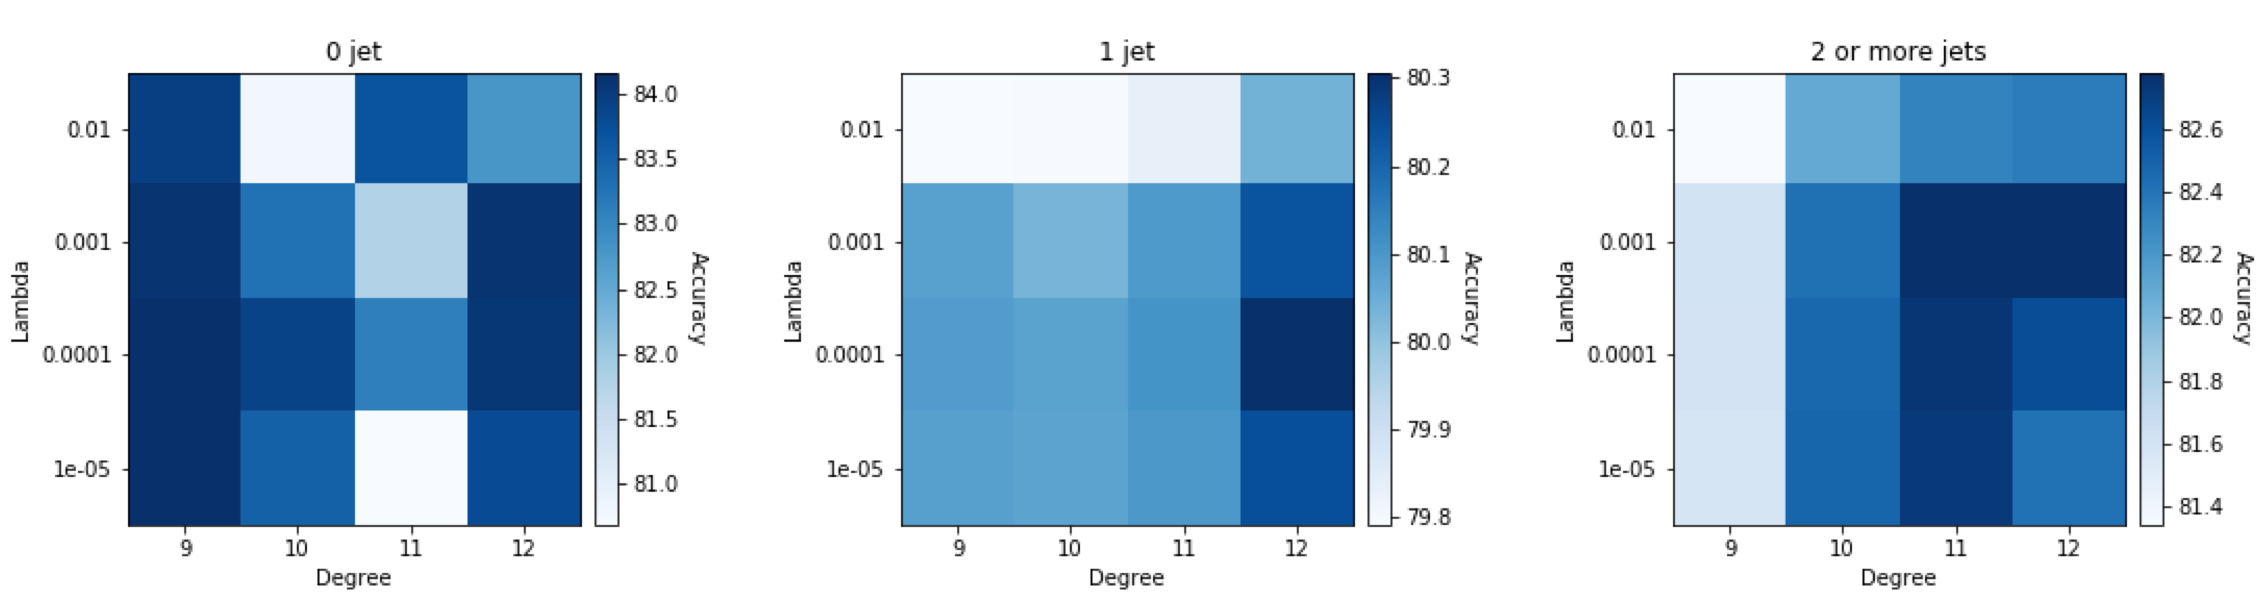
\includegraphics[scale=0.235]{best_parameters.png}
\caption{Hyperparameter optimization for model A: left to right, figures correspond to sets '0 jet', '1 jet' and '2+ jets' with the left $y$-axis, $x$-axis and right $y$-axis respectively the penalty tuner $\lambda$, the extension degree $n$ and the prediction score.}
\label{param}
\end{center}
\end{figure}


%Table 3: Performance score per model
\begin{table}[]
    \centering
    \caption{Prediction scores for each sub-set and model.}
    \label{tab:subset}
    \begin{tabular}{|c|c|c|c|}
    \hline
    \textbf{Model} &  '0 jet' &  '1 jet'  & '2+ jets' \\
    \hline
    \textbf{A} & 0.84171 & 0.80306 & 0.82781 \\
    \hline
    \textbf{B} & ... & ... & ... \\
    \hline
     \textbf{C} & 0.82374 & 0.75944 & 0.76174 \\
    \hline
    \end{tabular}
    \vfill
\end{table}

%Table 3: Hyperparameters optimization 
\begin{table}[]
    \centering
    \caption{Optimized hyperparameters for model A.}
    \label{tab:param}
    \begin{tabular}{|c|c|c|c|}
    \hline
     \textbf{Parameter} &  '0 jet' &  '1 jet' & '2+ jets'  \\
    \hline
    Degree $n$ & 9 & 12 & 12 \\
    \hline
     \textit{$\lambda$} & 1e-4 & 1e-4 & 1e-3  \\
    \hline
     \end{tabular}
     \vfill
\end{table}


%-----Discussion-----
\section{Discussion}
\label{sec:discussion}

-	What to improve? More into feature engineering, deeper understanding of the nature of the data, better feature augmentation: not only polynomial basis, but also logarithmic basis, square-roots basis, sinusoidal basis 
-	Check for more information about the correlation between features, which features are fundamental? Which carry very little information : at first we tried correlation matrix and PCA?  --> we did not spend much time on that because of the big number of data, possible to keep all of the features (rule of thumb 100 samples per parameter)
-	Ridge regression  good results, good computation time, limited as it is not a real binary classifier but a simple regression?
-	Logistic regression: transforms the prediction into a true probability: given the vector w we predict the probability of the class label 1 good for classification of binary problems looks good for our data set, need to make sure the labels -1  0 + long computational times, more complex especially for the big data set, implemented too late not the time to actually optimize it

%\section*{Acknowledgements}

%\bibliographystyle{IEEEtran}
%\bibliography{literature}

\end{document}